\section{Intelligence Artificielle}

\subsection{Stratégies}

\subsubsection{RandomAI}
Cette stratégie consiste en un joueur qui, à chaque étape du jeu, aurait le choix entre plusieurs options et en choisit une de manière aléatoire.

\subsubsection{HeuristicAI}
Dans l'intelligence heuristique, l'IA devra avoir un meilleur comportement qu'avec les commandes générées par le hasard. Ainsi, les choix faits par l'IA seront davantage réfléchis et permettront d'avancer d'une meilleure manière vers la fin du jeu et la défaite ou la victoire de l'un des deux joueurs. 
Pour chaque fonction, il est clair que de nombreuses stratégies existent pour jouer au Risk, que, dans une partie réelle, plusieurs d'entre-elles s'entremêlent inévitablement pour apporter le meilleur résultat possible au joueur. Dans notre cas, nous choisissons et expliquons une stratégie envisageable, réalisable pour notre jeu.
\newline

\begin{itemize}
    \item \textbf{aiRepartitionArmees.} 
    Dans cette fonction, l'IA doit choisir combien d'armées elle place sur chacun des territoires qui lui sont attribués. Pour trouver la meilleure méthode et stratégie, il convient de rappeler l'objectif du jeu. Pour l'instant, conquérir une certaine partie de la carte est l'objectif fixé : disons que le joueur gagnant devra posséder 28 territoires pour gagner (donc en conquérir 14). L'idée est donc de placer le plus d'armées sur les territoires qui ne sont pas trop isolés. En effet, posséder un réseau de pays sur lesquels les déplacements sont possibles permet de mieux structurer son attaque, effectuer des déplacements, mais aussi organiser sa défense.
    \newline
    
    \item \textbf{aiChoixPaysAttaquant.}
    Dans cette fonction, l'intelligence artificielle devra choisir le pays qu'elle possède avec le plus d'armées afin d'attaquer. Si plusieurs pays ont le même nombre d'armées, elle devra sélectionner celui qui est le plus en contact avec des états voisins appartenant au même joueur. Là encore, cette méthode permettra de renforcer les éventuelles pertes ou de ré-organiser la mise en place des armées en cas de défaite de l'attaque. 
    \newline
    
    \item \textbf{aiChoixPaysAttaque.}
   De manière très simple, nous choisissons d'attaquer le pays frontalier ennemi qui a le plus moins d'armées. Cela donne un pourcentage de chance plus important de remporter une attaque, et un éventuel territoire. Si plusieurs pays frontaliers ont le nombre d'armées minimum, on choisit le pays qui a le plus de frontaliers appartenant au joueur.
   \newline
   
   \item \textbf{aiNbDesAttaquant.}
    On rappelle que l'attaque ne peut pas attaquer en mettant en péril son territoire. De plus, le choix du nombre d'armées attaquantes, et de défense se fait en même temps, ainsi aucun des deux joueurs ne peut connaître le choix fait par son adversaire avant de choisir à son tour. 
    \newline
    L'attaquant peut choisir d'attaquer avec 1, 2 ou 3 armées. Lorsque c'est possible, le mieux est bien entendu d'attaquer avec trois armées puisque cela augmente la possibilité de réaliser un bon lancer de dés. Lorsque le joueur attaquant possède 4 armées ou plus, il choisit d'attaquer avec 3 armées. Sinon, il attaque avec une armée de moins que le nombre d'armées qu'il possède sur son territoire, soit le nombre maximal qui lui est autorisé.
    \newline
    
    \item \textbf{aiNbDesAttaque.}
    Dès que possible, l'IA défend avec 2 armées. Cela augmente ses chances de battre l'attaque, bien que le risque de perdre deux pions soit aussi présent. 
    Si le défenseur possède 2 armées ou plus sur le territoire, il défend avec 2. S'il ne possède qu'une armée, il défend avec son unique armée.
    \newline
    
    \item \textbf{aiDefausser.}
    Le joueur compte combien de cartes de chaque "force" (TANK, CANON ou SOLDAT) il possède et décide de la meilleure carte à défausser en fonction de s'il possède déjà trois cartes de même force (qu'il pourrait ainsi échanger contre des armées) et du gain que rapporte chaque combinaison de cartes (les soldats rapportant moins que les canons ou les tanks, ils seront les premiers à être défaussés). Ainsi, selon les cartes que le joueur possède, il défaussera une carte selon ce tableau :
    \begin{figure}[!htbp]
        \centering
        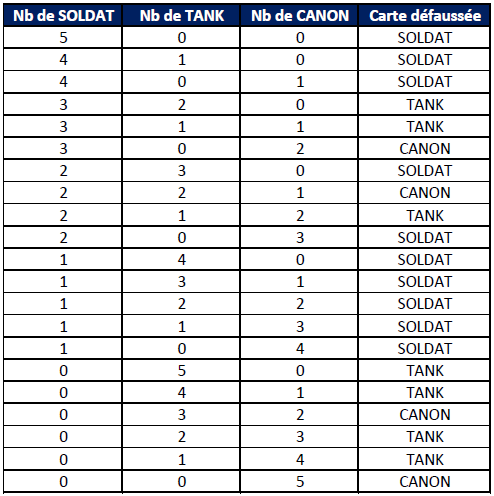
\includegraphics[width=7cm]{Images/defausse.png}
        \caption{Carte défaussée en fonction de la main du joueur}
        \label{fig:defausse}
    \end{figure}
    
    \item \textbf{aiEchange.}
    Dès que le joueur a trois cartes de même "force", il décide automatiquement de les échanger contre des armées.
    \newline
    
    \item \textbf{aiPlacerNouvellesArmees.}
    Lorsque le joueur doit placer de nouvelles armées à la fin de son tour, il choisit de les placer sur ses territoires possédant le moins d'armées.
    \newline
    
    \item \textbf{aiDéplacerArmees.}
    Plusieurs déplacements sont très intéressants à effectuer. Si le joueur possède un territoire entièrement entouré par des territoires amis, alors on ne peut laisser qu'une unique armée dessus (il ne peut êter attaqué) et ainsi renforcer les défenses alentours. 
\end{itemize}

\subsubsection{DeepAI}
Cette intelligence reprend certaines fonctions de l'intelligence heuristique. Nous donnons deux options de pays attaquant avec chacun deux options de pays attaqué (choisis selon les critères de l'heuristique). Chaque option est essayée et retire un certain nombre de points, calculés en fonction du nombre d'armées et de terrains controllés à l'issue de plusieurs tours de jeu potentiels. Ces points sont déterminés par l'algorithme du min/max basé sur le fait que le joueur veut maximiser ses gains alors que son adversaire va tenter de les minimiser. 
\newline

\subsection{Conception logiciel}
Le diagramme des classes pour l’intelligence artificielle est présenté en figure \ref{fig:ai}.

\textbf{Les Classes AI} : Les classes héritières de AI implémentent plusieurs stratégies d'intelligence artificielle.
\begin{itemize}
    \item RamdomAI : Intelligence aléatoire
    \item HeuristicAI : Intelligence heuristique
    \item DeepAI : Intelligence approfondie
\end{itemize}

\begin{landscape}
    \begin{figure}[!htbp]
        \centering
        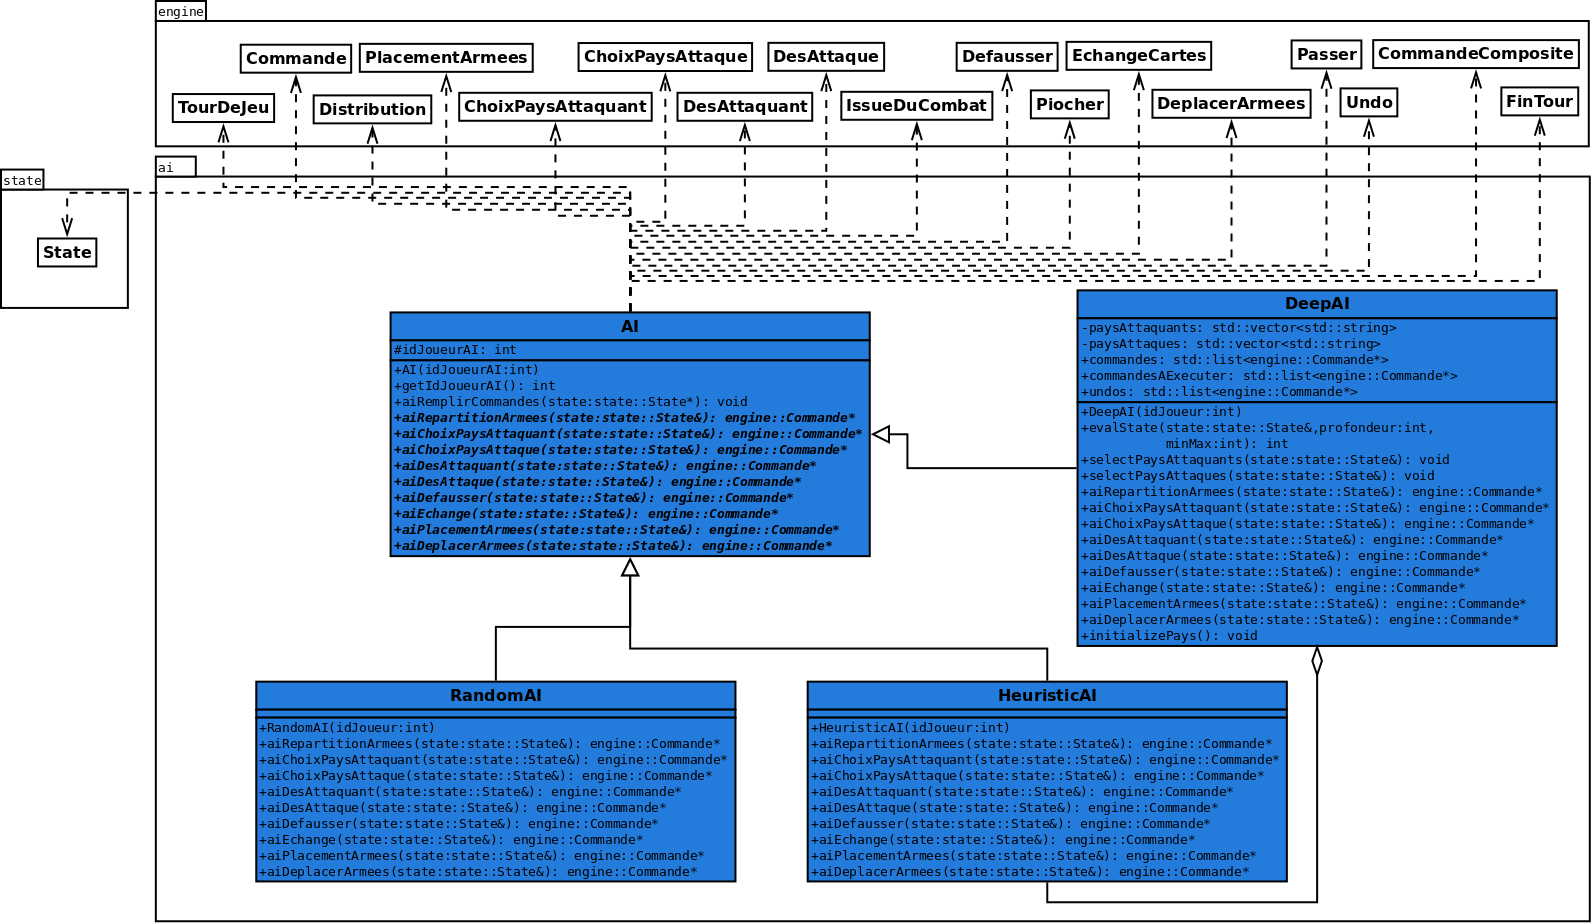
\includegraphics[width=17cm]{Images/ai.png}
        \caption{Diagramme de l'intelligence artificielle}
        \label{fig:ai}
    \end{figure}
\end{landscape}

